\documentclass[11pt,oneside]{scrbook}
\usepackage[a4paper,margin=2.4cm,marginparwidth=1.8cm,marginparsep=0.4cm]{geometry}
\usepackage{../common/rlstudy}

\title{{\color{rlblue}\textbf{Week 10} \\ \Huge SAC, TD3, and CrossQ for Continuous Control}}
\author{STUDY-RL --- a self-paced Deep RL curriculum}
\date{\today}

\begin{document}
\maketitle
\tableofcontents
\newpage

\chapter*{Learning objectives}
\addcontentsline{toc}{chapter}{Learning objectives}


% Teaching companion: a small example before the full lecture.
\noindent\textbf{Study companion.} Read \texttt{teaching\_guide.md} in this
folder for step-by-step examples, an analogy with its limits, and self-checks.
Then use \texttt{workbook.ipynb} to implement and vary the calculations.
\par\medskip

\begin{keyidea}
By the end of this week you will be able to:
\begin{enumerate}[leftmargin=*]
  \item Contrast stochastic and deterministic policy families and identify when each yields a lower-variance gradient.
  \item Derive the SAC (soft actor-critic) objective from the maximum-entropy MDP formulation; state the soft Bellman equations and the closed-form soft policy.
  \item Implement the tanh-squashed Gaussian policy, including the Jacobian correction to its log-density, and explain why the correction is essential.
  \item Train SAC on Pendulum-v1 (or MuJoCo Hopper) with automatic temperature tuning; plot return and entropy.
  \item Specify TD3 (twin critics, target policy smoothing, delayed updates) and explain its role as the deterministic-policy counterpart to SAC.
  \item Summarise CrossQ (2024) and the SimBa block (2025) as the off-policy continuous-control SOTA, including why CrossQ drops target networks.
\end{enumerate}
\end{keyidea}

\chapter{Motivation and intuition}

PPO is on-policy: it reuses each rollout for several optimisation epochs, then normally replaces it with fresh data. For continuous control with expensive simulators (or robots), this is a luxury. \marginnote{Throughput rule of thumb: SAC at UTD=1 sees the same data 8--16 times via the replay buffer; CrossQ at UTD=2 amortises each transition $\sim$32 times. On a single GPU you can typically get 10--50$\times$ more sample-efficient learning out of off-policy than on-policy methods.} Off-policy methods --- SAC, TD3, and the modern ensemble variants --- amortise every transition across many gradient updates through a replay buffer, and they exploit the reparameterisation trick (week 7) to compute low-variance pathwise gradients for the actor.

\begin{intuition}
SAC and TD3 are duals.
\begin{itemize}[leftmargin=*]
  \item TD3 trains a \emph{deterministic} policy $a = \mu_\theta(s)$. Exploration comes from Gaussian noise added to actions at \emph{rollout} time, not from the policy itself. Stability tricks: twin critics, delayed actor updates, target-action smoothing.
  \item SAC trains a \emph{stochastic} policy $\Policy_\theta(a\given s) = \tanh(\mathcal{N}(\mu_\theta(s), \sigma_\theta(s)^2))$. Exploration is a property of the policy itself. The critic learns the soft Q-function; the actor maximises a soft-Bellman-corrected entropy-regularised objective.
\end{itemize}
Both train two critics and use target networks; both update the actor by gradient descent through the critic (pathwise gradient).
\end{intuition}

\begin{pitfall}
The single most common bug in a SAC implementation is forgetting the tanh-Jacobian correction in the log-probability. The policy will then silently collapse to a near-deterministic edge of the action space, scoring artificially high entropy reported by the un-corrected formula. Verify the density, not its logarithm: $\int_{-1}^{1}\Policy(a\given s)\,da=1$. For one action dimension and $U\sim\mathrm{Uniform}(-1,1)$, $2\E[\exp(\log\Policy(U\given s))]=1$; numerical quadrature is another check.
\end{pitfall}

\chapter{Mathematical formulation}

\section{Stochastic vs.\ deterministic policies}

\paragraph{Stochastic policy gradient (score-function form):}
$\nabla_\theta J = \E[\nabla_\theta \log \Policy_\theta(a\given s)\, \Qfn^\Policy(s,a)]$.

\paragraph{Deterministic policy gradient (Silver 2014):}
\begin{theorem}[DPG]
\label{thm:dpg}
For a deterministic policy $a = \mu_\theta(s)$ and a state distribution $d^\mu$,
\[
  \nabla_\theta J(\mu_\theta) = \E_{s \sim d^\mu}\!\left[\nabla_\theta \mu_\theta(s)\, \nabla_a \Qfn^{\mu_\theta}(s, a)\big|_{a=\mu_\theta(s)}\right].
\]
\end{theorem}

\begin{proof}[Sketch]
Apply the chain rule to $J(\mu_\theta) = \E_{s\sim d^\mu}[\Qfn^{\mu_\theta}(s,\mu_\theta(s))]$. The expectation is over a parameter-dependent $d^\mu$, but the same Bellman-flow trick as in the stochastic PG theorem cancels the implicit $\partial d^\mu/\partial \theta$ contribution; the surviving term is exactly the chain rule applied to the inner $\Qfn(s,\mu_\theta(s))$.
\end{proof}

The deterministic gradient has lower variance (it averages out the exploration noise of the stochastic version) but requires the action space to be continuous and the critic to be differentiable in $a$.

\section{Maximum entropy RL}

The classical RL objective $J(\theta) = \E[\sum_t \Disc^t r_t]$ is augmented to
\[
  J_\text{MaxEnt}(\theta) = \E\!\left[\sum_t \Disc^t \big(r_t + \alpha \mathcal{H}(\Policy_\theta(\cdot\given s_t))\big)\right],
\]
with $\alpha \ge 0$ the temperature. The optimal policy is no longer deterministic; it is the Gibbs distribution over actions weighted by Q.

\begin{theorem}[Soft Bellman equations, Haarnoja 2018a]
\label{thm:soft}
For the entropy-regularised MDP, the soft value function $\Vfn^\Policy(s) = \E_{a\sim\Policy}[\Qfn^\Policy(s,a) - \alpha \log \Policy(a\given s)]$, and the soft Bellman backup
\[
  \mathcal{T}^\Policy \Qfn(s, a) \;=\; r(s, a) + \Disc\, \E_{s'}\!\left[\E_{a'\sim\Policy}\!\big[\Qfn(s', a') - \alpha \log \Policy(a'\given s')\big]\right].
\]
The soft-optimal policy is the Boltzmann form $\Policy^\star(a\given s) \propto \exp(\Qfn^\star(s,a)/\alpha)$.
\end{theorem}

\begin{proof}[Derivation of the optimal policy]
At fixed $\Qfn$, the actor update solves
\[
  \Policy^\text{new}(\cdot\given s) = \argmax_\Policy \E_{a\sim\Policy}[\Qfn(s,a)] + \alpha \mathcal{H}(\Policy(\cdot\given s)).
\]
Lagrangian on the simplex $\int \Policy(a\given s)\, da = 1$:
\[
  \mathcal{L}(\Policy, \nu) = \int \Policy(a\given s)\, \Qfn(s,a)\, da - \alpha \int \Policy \log \Policy\, da - \nu \big(\int \Policy\, da - 1\big).
\]
Functional derivative: $\delta\mathcal{L}/\delta \Policy = \Qfn(s,a) - \alpha (\log \Policy + 1) - \nu = 0$. Solving, $\Policy(a\given s) = \exp((\Qfn(s,a) - \nu - \alpha)/\alpha)$, and normalising gives the Boltzmann form. The result $\Vfn = \alpha \log \int \exp(\Qfn/\alpha)\, da$ is the soft-max (log-sum-exp) over actions.
\end{proof}

\section{Tanh-squashed Gaussian + Jacobian correction}

We need a stochastic policy that:
\begin{enumerate}[leftmargin=*]
  \item samples in a bounded box $[-1, 1]^{|\Actions|}$ (continuous-control envs require this);
  \item is differentiable through the sample (reparameterisable);
  \item has a tractable density.
\end{enumerate}

The standard recipe: $u \sim \mathcal{N}(\mu_\theta(s), \sigma_\theta(s)^2)$, then $a = \tanh(u)$. By the change-of-variables formula,
\[
  \Policy(a\given s) = \mathcal{N}(u; \mu, \sigma^2) \cdot \left|\frac{du}{da}\right|.
\]
Since $u=\tanh^{-1}(a)$, $du/da=1/(1-a^2)$, while $da/du=1-\tanh^2(u)$. Taking logarithms gives
\[
  \log \Policy(a\given s) = \log \mathcal{N}(u; \mu, \sigma^2) - \sum_{i=1}^{|\Actions|} \log(1 - a_i^2).
\]
Numerically, $\log(1-\tanh^2 u) = 2(\log 2 - u - \mathrm{softplus}(-2u))$ is stable.

\begin{pitfall}
Drop the Jacobian and your policy will report $\log\Policy$ that is artificially \emph{lower} (because $\tanh$ compresses); the entropy bonus $-\alpha \log\Policy$ in the actor loss becomes artificially high; the policy will push to the boundary of the action space and saturate. The optimiser will not crash; it will silently converge to a wrong policy.
\end{pitfall}

\section{Automatic temperature tuning}

Haarnoja 2018b makes $\alpha$ a learned parameter by enforcing the constraint
\[
  \E_{a \sim \Policy_\theta}[-\log \Policy_\theta(a\given s)] \ge \mathcal{H}_\text{target} = -|\Actions|.
\]
The dual update is
\[
  \alpha \leftarrow \alpha - \eta_\alpha \nabla_\alpha\, \alpha \cdot \big(-\log \Policy_\theta(a\given s) - \mathcal{H}_\text{target}\big),
\]
implemented by storing $\log\alpha$ unconstrained and computing $\alpha = \exp(\log\alpha)$. This removes the brittle $\alpha$ hyperparameter and is the single biggest reason SAC is the default off-policy baseline.

\section{TD3}

Twin Delayed DDPG (Fujimoto 2018) fixes three pathologies of DDPG:
\begin{enumerate}[leftmargin=*]
  \item \textbf{Overestimation bias.} Train two critics $\Qfn_{\phi_1}, \Qfn_{\phi_2}$; the target uses $\min(\Qfn_{\phi_1'}, \Qfn_{\phi_2'})$.
  \item \textbf{Function-approximation error in actor target.} Delay actor updates: update the actor every $d=2$ critic steps.
  \item \textbf{Deterministic-policy target sharpness.} Smooth the target action: $a' = \mu_{\theta'}(s') + \mathrm{clip}(\epsilon, -c, c)$, $\epsilon \sim \mathcal{N}(0, \tilde\sigma^2)$.
\end{enumerate}

The TD3 target is
\[
  y = r + \Disc \min_{i=1,2} \Qfn_{\phi_i'}(s', a'), \quad a' = \mu_{\theta'}(s') + \mathrm{clip}(\epsilon, -c, c).
\]

\section{CrossQ (2024) --- target nets considered harmful}

Bhatt et al.\ (ICLR 2024) show that with careful BatchNorm placement (BN after every Linear, both critics, train mode during the target computation too), the polyak-averaged target nets can be dropped without instability. Practical gain: $\sim$25\% wall-clock improvement and one fewer hyperparameter. The SimBa block (Lee et al.\ ICLR 2025) builds on this with residual + LayerNorm + RMSNorm and pushes the SOTA further on DMC.

\chapter{Algorithms}

\begin{tcolorbox}[colback=rlbg, colframe=rlblue, title=\textbf{SAC with automatic temperature}]
\textbf{Hyper-params:} replay buffer $D$ of size $10^6$, batch $B=256$, $\Disc=0.99$, polyak $\tau=5\times 10^{-3}$, actor/critic lr $=3\times 10^{-4}$, $\alpha$-lr $=3\times 10^{-4}$, $\mathcal{H}_\text{target} = -|\Actions|$.\\
\textbf{Init:} actor $\Policy_\theta$, critics $\Qfn_{\phi_1}, \Qfn_{\phi_2}$ and their polyak copies $\Qfn_{\phi_1'}, \Qfn_{\phi_2'}$.\\
\textbf{For each env step:}
\begin{enumerate}[leftmargin=*]
  \item Sample $a \sim \Policy_\theta(\cdot\given s)$, step env, store $(s, a, r, s', d)$.
  \item Sample minibatch $\sim D$.
  \item Compute target: $\tilde a \sim \Policy_\theta(\cdot\given s')$, $\log\tilde p = \log\Policy_\theta(\tilde a\given s')$,
        \[
          y = r + \Disc (1-d)\big[\min_i \Qfn_{\phi_i'}(s', \tilde a) - \alpha \log\tilde p\big].
        \]
  \item Critic update: minimise $\sum_i (\Qfn_{\phi_i}(s,a) - y)^2$.
  \item Actor update (reparameterised): minimise $\E[\alpha \log\Policy_\theta(a\given s) - \min_i \Qfn_{\phi_i}(s,a)]$.
  \item Temperature update: minimise $\E[-\alpha (\log\Policy_\theta(a\given s) + \mathcal{H}_\text{target})]$ in $\log\alpha$.
  \item Polyak update: $\phi_i' \leftarrow \tau \phi_i + (1-\tau)\phi_i'$.
\end{enumerate}
\end{tcolorbox}

\begin{tcolorbox}[colback=rlbg, colframe=rlblue, title=\textbf{TD3}]
\textbf{Hyper-params:} as SAC, plus action-noise $\sigma=0.1$, target-noise $\tilde\sigma=0.2$, noise clip $c=0.5$, delay $d=2$.\\
\textbf{For each env step:}
\begin{enumerate}[leftmargin=*]
  \item Roll out with $a = \mu_\theta(s) + \mathcal{N}(0, \sigma^2)$.
  \item Critic step (twin): target $y = r + \Disc \min_i \Qfn_{\phi_i'}(s', \mu_{\theta'}(s') + \mathrm{clip}(\epsilon, -c, c))$.
  \item Every $d$ steps: actor step ($\nabla_\theta \E[\Qfn_{\phi_1}(s, \mu_\theta(s))]$), then polyak update of all targets.
\end{enumerate}
\end{tcolorbox}

\chapter{Implementation walkthrough}

\section{Tanh-squashed Gaussian (the right way)}

\begin{minted}{python}
class TanhGaussianPolicy(nn.Module):
    def __init__(self, obs_dim, act_dim, hidden=(256, 256)):
        super().__init__()
        # mu and log_sigma heads share a trunk; both depend on s.
        self.trunk = mlp([obs_dim, *hidden], output_activation=nn.ReLU)
        self.mu = nn.Linear(hidden[-1], act_dim)
        self.log_sigma = nn.Linear(hidden[-1], act_dim)

    def sample(self, obs):
        z = self.trunk(obs)
        mu = self.mu(z)
        log_sigma = self.log_sigma(z).clamp(-5, 2)
        sigma = log_sigma.exp()
        eps = torch.randn_like(mu)
        u = mu + sigma * eps
        a = torch.tanh(u)
        # log N(u; mu, sigma^2) - sum log(1 - a^2)  (numerically stable form)
        log_p_u = -0.5 * (((u - mu) / sigma) ** 2 + 2 * log_sigma
                          + math.log(2 * math.pi))
        # log|da/du|^-1 = -log(1 - tanh^2 u); stable form:
        log_det_jac = 2.0 * (math.log(2.0) - u - F.softplus(-2.0 * u))
        log_prob = (log_p_u - log_det_jac).sum(-1)
        return a, log_prob
\end{minted}

\section{SAC critic update}

\begin{minted}{python}
def critic_update(batch, actor, q1, q2, q1_tgt, q2_tgt, log_alpha,
                  gamma=0.99, opt=None):
    s, a, r, s2, d = batch
    with torch.no_grad():
        a2, logp2 = actor.sample(s2)
        q_tgt = torch.min(q1_tgt(s2, a2), q2_tgt(s2, a2)) - log_alpha.exp() * logp2
        y = r + gamma * (1 - d) * q_tgt
    L = ((q1(s, a) - y) ** 2 + (q2(s, a) - y) ** 2).mean()
    opt.zero_grad(); L.backward(); opt.step()
\end{minted}

\chapter{Empirical results}

\begin{figure}[h]
\centering
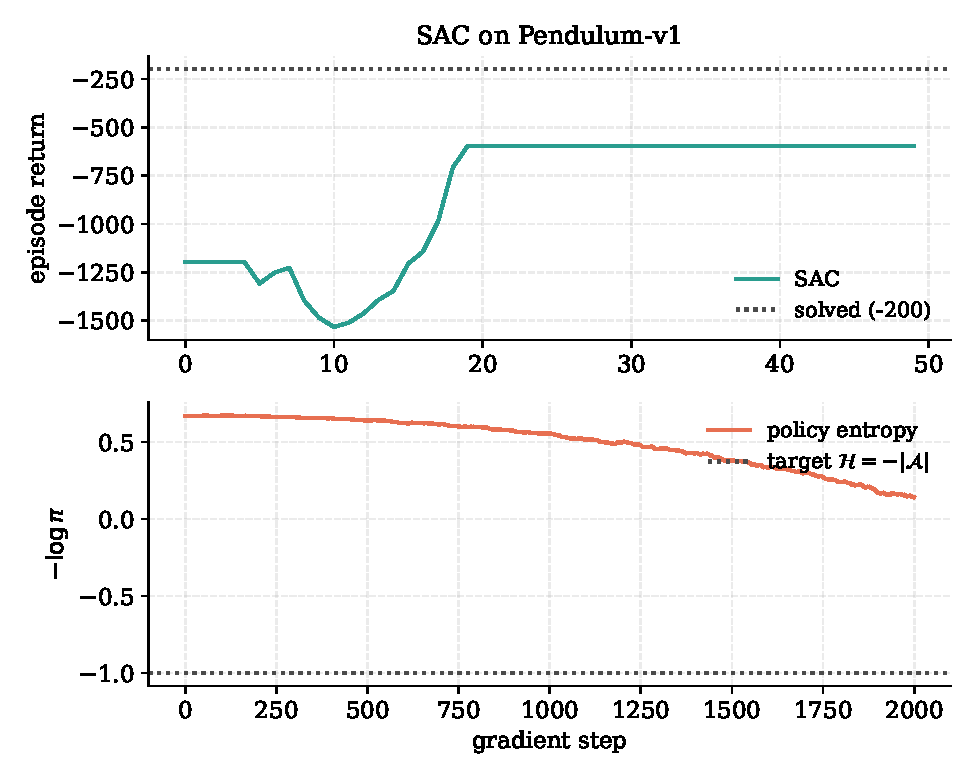
\includegraphics[width=0.85\linewidth]{figs/sac_pendulum.pdf}
\caption{SAC on Pendulum-v1. Three seeds; return (top) and policy entropy (bottom). Note that the entropy decreases during training as the policy becomes more confident; with automatic temperature tuning, it stabilises near the target $-|\Actions| = -1$.}
\label{fig:sac-pendulum}
\end{figure}

\chapter{Safety angle}

\begin{safetyangle}
\textbf{Three failure modes that matter for high-stakes off-policy RL.}

\begin{enumerate}[leftmargin=*]
  \item \textbf{Q-function over-estimation cascade.} A single mis-fit batch can push $\Qfn(s,a)$ several units too high; the next policy update will increase the probability of that action, generating more high-$\Qfn$ data, generating more upward bias. The twin-critic min trick of TD3/SAC is the structural fix. \emph{Watch the empirical $\min_i \Qfn_i$ during training}; a runaway uptrend is the failure signature.
  \item \textbf{Stuck entropy.} If the automatic temperature update is mis-coded (most commonly: forgetting that the temperature loss should be a function of $\log\alpha$ not $\alpha$), the policy entropy either explodes or collapses. Mitigation: clamp $\log\alpha \in [-5, 2]$ and assert the gradient sign is correct in unit tests.
  \item \textbf{Replay-buffer drift.} On long runs ($> 10^6$ steps) the buffer contains transitions from radically different past policies. The Q-targets become biased. This is exactly the setting where \emph{constrained safe RL} (week 16) needs explicit safety filters; the off-policy bias compounds with reward mis-specification to produce non-monotone training.
\end{enumerate}

\paragraph{Matching context.}
For an off-policy matching system retrained nightly on the day's logs, the entropy-regularised objective is structurally useful: it prevents the policy from collapsing onto a single broker / candidate / item even when the reward signal degenerates. The same maximum-entropy principle is the rationale for the KL-to-reference term in RLHF (week 18); the only difference is that there the ``reference'' is a fixed prior policy, while in SAC it is the uniform distribution.
\end{safetyangle}

\chapter{Matching application}

\begin{matching}
\textbf{SAC as the nightly retrainer for synthetic ATS candidate-ranking.}

The matching setting in production usually has continuous-valued match-quality features and is too high-dimensional for tabular methods. SAC fits naturally:
\begin{itemize}
  \item \textbf{State $s$:} candidate embedding (768-dim), job-pool snapshot (256-dim).
  \item \textbf{Action $a \in \Real^d$:} score adjustments over the top-100 candidates (so $|\Actions|=100$, then we softmax-sample the top-K).
  \item \textbf{Reward $r$:} hire-conversion within 30 days, possibly normalised by base rate.
  \item \textbf{Replay buffer $D$:} 90 days of logged $(s, a, r, s')$.
\end{itemize}

The automatic temperature tuning is particularly valuable here: it removes the need to manually trade off exploration (showing new candidates) vs.\ exploitation (showing the model's favourites). The maximum-entropy objective keeps the candidate-shortlisting policy diverse, which encourages diversity but provides no individual or group fairness guarantee; an entropy bonus can coexist with severe exposure disparities.

\paragraph{Operational caveats.}
\begin{itemize}
  \item Production deployment requires a CMDP layer (week 16) to enforce hard fairness constraints (e.g.\ minimum exposure per demographic group). SAC alone is the optimiser; it does not provide guarantees.
  \item Replay-buffer drift over the 90-day window is a real concern; in practice we re-fit the value head weekly from scratch on the most recent two weeks to combat this.
\end{itemize}
\end{matching}

\chapter{Exercises}

\begin{enumerate}[label={},leftmargin=0pt,labelsep=0pt]
  \item \textbf{E1} ($\star$) Verify the tanh-Jacobian correction: sample $u \sim \mathcal{N}(0, 1)$, transform to $a=\tanh u$, compute the corrected $\log\Policy(a)$, and check that the density $\exp(\log\Policy(a))$ integrates to $1$ over $(-1,1)$.
  \item \textbf{E2} ($\star$) Derive the soft-optimal policy in closed form via the Lagrangian and confirm $\Policy^\star \propto \exp(\Qfn/\alpha)$.
  \item \textbf{E3} ($\star\star$) Implement the SAC critic update for Pendulum and verify the loss decreases over 200 steps.
  \item \textbf{E4} ($\star\star$) Implement the actor reparameterised loss; verify the gradient sign on a toy 1-d problem.
  \item \textbf{E5} ($\star\star$) Implement automatic temperature tuning; show that $\alpha$ converges to a value that yields $\mathcal{H} \approx \mathcal{H}_\text{target}$.
  \item \textbf{E6} ($\star\star$) Train SAC on Pendulum-v1 to a smoothed return $\ge -200$ within 8000 env steps.
  \item \textbf{E7} ($\star\star\star$) Code TD3 in $\sim$100 lines; compare wall-clock to SAC on Pendulum.
  \item \textbf{E8} ($\star\star\star$, meaningful objective) For a logged-bandit matching dataset, run an off-policy SAC variant: load the logs into the replay buffer and train without env interaction. Verify that the resulting policy beats the behaviour policy in SNIPS-estimated value.
\end{enumerate}

\chapter{Further reading}

See \texttt{extended\_reading.pdf}. Five papers: Lillicrap et al.\ 2015 (DDPG), Fujimoto et al.\ 2018 (TD3), Haarnoja et al.\ 2018a/b (SAC + automatic temperature), Bhatt et al.\ 2024 (CrossQ), Lee et al.\ 2025 (SimBa). Sourced from \texttt{research/deeprl\_core\_sota.md} \S 3.1--3.7.

\end{document}
